% !TEX TS-program = xelatex
\documentclass[10pt,landscape,a4paper]{article}
%\usepackage[utf8]{inputenc}
%\usepackage[ngerman]{babel}
\usepackage[normalem]{ulem}
\usepackage{tikz}
\usetikzlibrary{shapes,positioning,arrows,fit,calc,graphs,graphs.standard}
\usepackage[nosf]{kpfonts}
\usepackage[t1]{sourcesanspro}
%\usepackage[lf]{MyriadPro}
%\usepackage[lf,minionint]{MinionPro}
\usepackage{multicol}
\usepackage{wrapfig}
\usepackage[top=0mm,bottom=1mm,left=0mm,right=1mm]{geometry}
\usepackage[framemethod=tikz]{mdframed}
\usepackage{microtype}
%\usepackage{physics}
\usepackage{tabularx}
\usepackage{hhline}
\usepackage{makecell}
\usepackage{mathtools}

\usepackage{listings}
\usepackage{mips}
\lstset{language=[mips]Assembler}

\DeclarePairedDelimiter{\ceil}{\lceil}{\rceil}

\newcommand\codeblue[1]{\textcolor{blue}{\code{#1}}}

\usepackage{lastpage}
\usepackage{datetime}
\yyyymmdddate
\renewcommand{\dateseparator}{-}
\let\bar\overline

\definecolor{myblue}{cmyk}{1,.72,0,.38}

\def\firstcircle{(0,0) circle (1.5cm)}
\def\secondcircle{(0:2cm) circle (1.5cm)}

\colorlet{circle edge}{myblue}
\colorlet{circle area}{myblue!5}

\tikzset{filled/.style={fill=circle area, draw=circle edge, thick},
    outline/.style={draw=circle edge, thick}}

\pgfdeclarelayer{background}
\pgfsetlayers{background,main}

%\everymath\expandafter{\the\everymath \color{myblue}}
%\everydisplay\expandafter{\the\everydisplay \color{myblue}}


\renewcommand{\baselinestretch}{.8}
\pagestyle{empty}

\global\mdfdefinestyle{header}{%
linecolor=gray,linewidth=1pt,%
leftmargin=0mm,rightmargin=0mm,skipbelow=0mm,skipabove=0mm,
}

\newcommand{\header}{
\begin{mdframed}[style=header]
\footnotesize
\sffamily
CS2100 Finals Cheatsheet v1.3 (\today)\\
by~Julius Putra Tanu Setiaji,~page~\thepage~of~\pageref{LastPage}
\end{mdframed}
}
%\usepackage{chngcntr}

\usepackage{verbatim}

\usepackage{etoolbox}
\makeatletter
\preto{\@verbatim}{\topsep=0pt \partopsep=0pt }
\makeatother

\counterwithin*{equation}{section}
\counterwithin*{equation}{subsection}
\usepackage{enumitem}
\newlist{legal}{enumerate}{10}
\setlist[legal]{label*=\arabic*.,leftmargin=2.5mm}
\setlist[itemize]{leftmargin=3mm}
\setlist[enumerate]{leftmargin=3mm}
\setlist{nosep}
\usepackage{minted}

\def\code#1{\texttt{#1}}

\newenvironment{descitemize} % a mixture of description and itemize
{\begin{description}[leftmargin=*,before=\let\makelabel\descitemlabel]}
	{\end{description}}

\newcommand{\descitemlabel}[1]{%
	\textbullet\ \textbf{#1}%
}
\makeatletter



\renewcommand{\section}{\@startsection{section}{1}{0mm}%
                                {.2ex}%
                                {.2ex}%x
                                {\color{myblue}\sffamily\small\bfseries}}
\renewcommand{\subsection}{\@startsection{subsection}{1}{0mm}%
                                {.2ex}%
                                {.2ex}%x
                                {\sffamily\bfseries}}
\renewcommand{\subsubsection}{\@startsection{subsubsection}{1}{0mm}%
                                {.2ex}%
                                {.2ex}%x
                                {\rmfamily\bfseries}}



\def\multi@column@out{%
   \ifnum\outputpenalty <-\@M
   \speci@ls \else
   \ifvoid\colbreak@box\else
     \mult@info\@ne{Re-adding forced
               break(s) for splitting}%
     \setbox\@cclv\vbox{%
        \unvbox\colbreak@box
        \penalty-\@Mv\unvbox\@cclv}%
   \fi
   \splittopskip\topskip
   \splitmaxdepth\maxdepth
   \dimen@\@colroom
   \divide\skip\footins\col@number
   \ifvoid\footins \else
      \leave@mult@footins
   \fi
   \let\ifshr@kingsaved\ifshr@king
   \ifvbox \@kludgeins
     \advance \dimen@ -\ht\@kludgeins
     \ifdim \wd\@kludgeins>\z@
        \shr@nkingtrue
     \fi
   \fi
   \process@cols\mult@gfirstbox{%
%%%%% START CHANGE
\ifnum\count@=\numexpr\mult@rightbox+2\relax
          \setbox\count@\vsplit\@cclv to \dimexpr \dimen@-1cm\relax
\setbox\count@\vbox to \dimen@{\vbox to 1cm{\header}\unvbox\count@\vss}%
\else
      \setbox\count@\vsplit\@cclv to \dimen@
\fi
%%%%% END CHANGE
            \set@keptmarks
            \setbox\count@
                 \vbox to\dimen@
                  {\unvbox\count@
                   \remove@discardable@items
                   \ifshr@nking\vfill\fi}%
           }%
   \setbox\mult@rightbox
       \vsplit\@cclv to\dimen@
   \set@keptmarks
   \setbox\mult@rightbox\vbox to\dimen@
          {\unvbox\mult@rightbox
           \remove@discardable@items
           \ifshr@nking\vfill\fi}%
   \let\ifshr@king\ifshr@kingsaved
   \ifvoid\@cclv \else
       \unvbox\@cclv
       \ifnum\outputpenalty=\@M
       \else
          \penalty\outputpenalty
       \fi
       \ifvoid\footins\else
         \PackageWarning{multicol}%
          {I moved some lines to
           the next page.\MessageBreak
           Footnotes on page
           \thepage\space might be wrong}%
       \fi
       \ifnum \c@tracingmulticols>\thr@@
                    \hrule\allowbreak \fi
   \fi
   \ifx\@empty\kept@firstmark
      \let\firstmark\kept@topmark
      \let\botmark\kept@topmark
   \else
      \let\firstmark\kept@firstmark
      \let\botmark\kept@botmark
   \fi
   \let\topmark\kept@topmark
   \mult@info\tw@
        {Use kept top mark:\MessageBreak
          \meaning\kept@topmark
         \MessageBreak
         Use kept first mark:\MessageBreak
          \meaning\kept@firstmark
        \MessageBreak
         Use kept bot mark:\MessageBreak
          \meaning\kept@botmark
        \MessageBreak
         Produce first mark:\MessageBreak
          \meaning\firstmark
        \MessageBreak
        Produce bot mark:\MessageBreak
          \meaning\botmark
         \@gobbletwo}%
   \setbox\@cclv\vbox{\unvbox\partial@page
                      \page@sofar}%
   \@makecol\@outputpage
     \global\let\kept@topmark\botmark
     \global\let\kept@firstmark\@empty
     \global\let\kept@botmark\@empty
     \mult@info\tw@
        {(Re)Init top mark:\MessageBreak
         \meaning\kept@topmark
         \@gobbletwo}%
   \global\@colroom\@colht
   \global \@mparbottom \z@
   \process@deferreds
   \@whilesw\if@fcolmade\fi{\@outputpage
      \global\@colroom\@colht
      \process@deferreds}%
   \mult@info\@ne
     {Colroom:\MessageBreak
      \the\@colht\space
              after float space removed
              = \the\@colroom \@gobble}%
    \set@mult@vsize \global
  \fi}
\global\let\tikz@ensure@dollar@catcode=\relax

\def\mathcolor#1#{\@mathcolor{#1}}
\def\@mathcolor#1#2#3{%
	\protect\leavevmode
	\begingroup
	\color#1{#2}#3%
	\endgroup
}

\makeatother
\setlength{\parindent}{0pt}

\setminted{tabsize=2, breaklines}
% Remove belowskip of minted
\setlength\partopsep{-\topsep}


\newcolumntype{a}{>{\hsize=1.5\hsize}X}
\newcolumntype{b}{>{\hsize=.25\hsize}X}

\setlength\columnsep{1.5pt}
\setlength\columnseprule{0.1pt}
\begin{document}
\setlength{\abovedisplayskip}{0pt}
	\setlength{\belowdisplayskip}{0pt}

\scriptsize
\begin{multicols*}{4}
	\raggedcolumns
	\section{C Programming Language}
	\subsection{Data Types}
	\newcolumntype{a}{>{\hsize=0.25\hsize}X}
	\newcolumntype{b}{>{\hsize=1.5\hsize}X}
	\begin{tabularx}{\columnwidth}{|a|a|b|}
		\hline
		\textbf{Type} & \textbf{\texttt{sizeof}} & \textbf{range} \\
		\hline
		\texttt{int} & 4 bytes & 2s complement, $(-2^{31})$ to $(2^{31}-1)$ OR (-2,147,483,648 to 2,147,483,647) \\ \hline
		\texttt{float} & 4 bytes & 1-bit sign, 8-bit exponent (excess-127), 23-bit mantissa \\ \hline
		\texttt{double} & 8 bytes & 1-bit sign, 11-bit exponent (excess-1023), 52-bit mantissa \\ \hline
		\texttt{char} & 1 byte & ASCII (7 bits + 1 parity bit), A is 100 0001 \\ \hline
	\end{tabularx}
	Note that for mantissa there is an implicit leading bit 1
	\subsection{Format Specifiers}
	\begin{tabular}{|l|l|l|}
		\hline
		\texttt{\%f} & \texttt{float} & \texttt{scanf} \\ \hline
		\texttt{\%lf} & \texttt{double} & \texttt{scanf} \\ \hline
		\texttt{\%e} & scientific notation & \texttt{printf} \\ \hline
		\texttt{\%p} & pointers & \texttt{printf} \\ \hline
	\end{tabular}
	\subsection{Escape Sequences}
	\begin{tabular}{|l|l|}
		\hline
		\texttt{\textbackslash n} & new line \\ \hline
		\texttt{\textbackslash t} & tab \\ \hline
	\end{tabular}
	\begin{tabular}{|l|l|}
		\hline
		\texttt{\textbackslash "} & double-quote " \\ \hline
		\texttt{\%\%} & percent \% \\ \hline
	\end{tabular}
	\subsection{Pointers}
	\begin{itemize}
		\item New unary operators: \texttt{*} and \texttt{\&}
		\item Convention: \mintinline{C}{int *abc;} AND \mintinline{C}{void f(int *);}
	\end{itemize}
	\subsection{Functions}
	\begin{itemize}
		\item Function prototype (just the type): e.g. \mintinline{C}{void g(int, int);}
		\item Variable scoping: by \textbf{functions}
	\end{itemize}
	\subsection{Arrays}
	\begin{itemize}
		\item When initialised with fewer values than elements, the rest are initialised as 0 (for \mintinline{C}{int}).
		\item Equivalence: value: \mintinline{C}{*(arr+2) == arr[2]} and memory location: \mintinline{C}{arr + 2 == &arr[2]}
	\end{itemize}
	\subsection{String}
	\begin{itemize}
		\item An array of characters, terminated by a null character \mintinline{C}{'\0'} 
		\item Initialising: \mintinline{C}{char str[4] = "egg";} or \mintinline{C}{char str[4] = {'e', 'g', 'g', '\0'};}
		\item Read from stdin: \mintinline{C}{fgets(str, size, stdin); // reads until (size - 1) or '\n'} and \mintinline{C}{scanf("%s", str); // reads until whitespace}
			(note: \mintinline{C}{fgets} also reads in \mintinline{C}{'\n'})
			\item Print to stdout: \mintinline{C}{puts(str);} $\equiv$ \mintinline{C}{printf("%s\n", str);}
				\item String functions:
				\begin{itemize}
					\item \mintinline{C}{strlen(s)}: returns the no of chars in \mintinline{C}{s}
					\item \mintinline{C}{strcmp(s1, s2)}: compare ASCII val of correspndg chars, similar to Java \texttt{compareTo}
					\item \mintinline{C}{strncmp(s1, s2, n)}: compare first $n$ chars of s1 and s2
					\item \mintinline{C}{strcpy(s1, s2)}: copy the string pointed by s2 into array pointed by s1, returns s1. E.g. \mintinline{C}{char s[4]; strcpy(s, "asdfgh"); // s == {'a', 's', 'd', '\0'};}
					\item \mintinline{C}{strncpt(s1, s2, n)}: copy the first $n$ chars of s2 to s1
				\end{itemize}
			\end{itemize}
			\subsection{Structures}
			\begin{itemize}
				\item Structures allow grouping of heterogeneous members of different types.
				\item Assignment  \mintinline{C}{result2 = result1;} copies the entire structure.
				\item Passing structure to function: the entire structure is copied.
				\item Alternatively, to change original structure, one can use pointer. Syntactic sugar: \mintinline{C}{(*player_ptr).name == player_ptr->name;}
				\item E.g.:
			\end{itemize}
			\begin{minted}{C}
typedef struct {
	int day, month, year;
} date_t;
typedef struct {
	int stuNum;
	date_t birthday;
} student_t;
student_t s1 = {1049858, {31, 12, 2020}};
// s1.birthday.month == 2020
			\end{minted}
				\subsection{Code Compilation Process}
				C Program (.c) -> \textbf{Preprocessor} -> Preprocessed code (.i) -> \textbf{Compiler} -> Assembly code (.asm) -> \textbf{Assembler} -> Object code (.o) -> \textbf{Linker} -> Executable (.hex)
	\section{Numbering Systems}
	\subsection{Data Representation}
		\begin{itemize}
			\item 1 byte = 8 bits
			\item $n$ bits can represent up to $2^n$ values. Thus, to present $m$ values, $\ceil{\log_2m}$ is required
		\end{itemize}
	\subsection{Decimal to Binary Conversion}
		\begin{itemize}
			\item For whole numbers: repeated division-by-2 (look at remainder)
			\item For fractions: repeated multiplication-by-2 (look at "quotient")
		\end{itemize}
	\subsection{Representation of Signed Binary Numbers}
		\newcolumntype{c}{>{\hsize=0.4\hsize}X}
		\newcolumntype{d}{>{\hsize=0.6\hsize}X}
		\newcolumntype{e}{>{\hsize=0.5\hsize}X}
		\newcolumntype{f}{>{\hsize=0.5\hsize}X}
		\begin{tabularx}{\columnwidth}{|c|d|e|f|}
			\hline
			 & Negation & Range & Zeroes \\
			\hline
			Sign-and-Magnitude & invert the sign bit (leading bit) & $-(2^{n-1} - 1)$ to $2^{n-1} - 1$ & $+0_{10}$ and $-0_{10}$ \\ \hline
			1s Complement & invert all the bits & $-(2^{n-1} - 1)$ to $2^{n-1} - 1$ & $+0_{10}$ and $-0_{10}$ \\ \hline
			2s Complement & invert all the bits, then add 1 & $-2^{n-1}$ to $2^{n-1}-1$ & $+0_{10}$ \\ \hline
		\end{tabularx}
		For all of the above, the MSB (Most Significant Bit) represents sign.
		\subsubsection{Sign-and-Magnitude}
			\begin{itemize}
				\item Range (8-bit): $(1111$ $1111)$ to $(0111$ $1111) = -127_{10}$ to $+127_{10}$
				\item Zeroes: $0000$ $0000 = +0_{10}$ and $1000$ $0000 = -0_{10}$
				\item e.g. $(\mathcolor{red}{0}011$ $0100)_{sm} = +011$ $0100_2 = +52_{10}$, $(\mathcolor{red}{1}001$ $0011)_{sm} = -(001$ $0011)_2 = -(19)_{10}$
			\end{itemize}
		\subsubsection{1s Complement (Diminished Radix)}
			\begin{itemize}
				\item Negation: $-x=2^n -x-1$
				\item Range (8-bit): $(1000$ $0000)$ to $(0111$ $1111) = -127_{10}$ to $+127_{10}$
				\item Zeroes: $(0000$ $0000) = +0_{10}$ and $(1111$ $1111) = -0_{10}$
				\item e.g. $(0000$ $1110)_{1s} = (0000$ $1110)_2 = (14)_{10}$,
				$(1111$ $0001)_{1s} = -(0000$ $1110)_2 = -(14)_{10}$
			\end{itemize}
		\subsubsection{2s Complement (Radix complement)}
			\begin{itemize}
				\item Negation: $-x = 2^n - x$
				\item Range (8-bit): $(1000$ $0000) = -128_{10}$ to $(0111$ $1111) = +127_{10}$
				\item Zero: $(0000$ $0000) = +0_{10}$
				\item e.g. $(0000$ $1110)_{2s} = (0000$ $1110)_2 = (14)_{10}$,  $(1111$ $0010)_{2s} = -(0000$ $1110)_2 = -(14)_{10}$
			\end{itemize}
		\subsubsection{Excess-k}
			\begin{itemize}
				\item Also known as offset binary. Use 0000 to represent $-k$ (lowest number possible)
				\item For unsigned, with $n$-bit number, $k=2^{n-1}-1$
			\end{itemize}
		\subsubsection{Comparison}
		\newcolumntype{g}{>{\hsize=0.2\hsize}X}
		\newcolumntype{h}{>{\hsize=0.45\hsize}X}
		\begin{tabularx}{\columnwidth}{|g|h|h|h|h|}
			\hline
			\textbf{Value} & \textbf{Sign-\&-Magnitude} & \textbf{1s Complement} & \textbf{2s Complement} & \textbf{Excess-8} \\
			\hline
			+7 & 0111 & 0111 & 0111 & 1111 \\ \hline
			+6 & 0110 & 0110 & 0110 & 1110 \\ \hline
			+5 & 0101 & 0101 & 0101 & 1101 \\ \hline
			+4 & 0100 & 0100 & 0100 & 1100 \\ \hline
			+3 & 0011 & 0011 & 0011 & 1011 \\ \hline
			+2 & 0010 & 0010 & 0010 & 1010 \\ \hline
			+1 & 0001 & 0001 & 0001 & 1001 \\ \hline
			+0 & 0000 & 0000 & 0000 & 1000 \\ \hline
			-0 & 1000 & 1111 & -    & -    \\ \hline
			-1 & 1001 & 1110 & 1111 & 0111 \\ \hline
			-2 & 1010 & 1101 & 1110 & 0110 \\ \hline
			-3 & 1011 & 1100 & 1101 & 0101 \\ \hline
			-4 & 1100 & 1011 & 1100 & 0100 \\ \hline
			-5 & 1101 & 1010 & 1011 & 0011 \\ \hline
			-6 & 1110 & 1001 & 1010 & 0010 \\ \hline
			-7 & 1111 & 1000 & 1001 & 0001 \\ \hline
			-8 & -    & -    & 1000 & 0000 \\ \hline
		\end{tabularx}
			
		\subsection{Operation on binary numbers}
		Algo for \textbf{Subtraction}: $A - B = A + (-B)$\\
		Algo for \textbf{Overflow Check}: if MSB of first and second are the same, then MSB of resulting numbers must be the same too.
		\subsubsection{2s Complement on Addition}
		Algo: Perform binary addition; Ignore the carry out of the MSB; Check for overflow.
\begin{verbatim}
Example, 2s Complement 4-bit
+3  0011          -2    1110          -3     1101
+4  0100          -6    1010          -6     1010
--- -----        ---   -----         ---    -----
+7  0111 (No of)  -8 (1)1000 (No of)  -9  (1)0111 (Of!)
\end{verbatim}
		\subsubsection{1s Complement on Addition}
		Algo: Perform binary addition; If there is carry out of the MSB, add 1 to the result; Check for overflow.
\begin{verbatim}
Example, 1s Complement 4-bit
+3  0011          -2    1101          -3     1100
+4  0100          -5    1010          -6     1001
--- -----        ---   -----         ---    -----
+7  0111 (No of)  -7 (1)0111          -9  (1)0101
                           1                    1
                       -----                -----
                        1000 (No of)   0110 (Of!)
\end{verbatim}
		\subsection{Floating Point}
		\begin{itemize}
			\item Single precision 32 bits: 1-bit sign, 8-bit exponent (excess-127), 23-bit mantissa
			\item Double precision 64 bits: 1-bit sign, 11-bit exponent (excess-1023), 52-bit mantissa
			\item e.g. $-6.5_{10} = -110.1_{2} = -1.101_{2} \times 2^2$, Exponent (excess-127) $= 2 + 127 = 129 = 1000$ $0001_2$
		\end{itemize}
			
\begin{verbatim}
Sign Exponent          Mantissa
 1   10000001 10100000000000000000000
\end{verbatim}
Hence, $1100$ $0000$ $1101$ $0000$ $0000$ $0000$ $0000$ $0000_2 = C0D0 0000_{16}$ (as \texttt{float}$ = -6.5$, as \texttt{int}$ = -1,060,110,336$)


	\section{MIPS}
	\subsection{Loading a 32-bit constant into a register}
		\begin{enumerate} 
			\item Use \texttt{lui} to set the upper 16-bit: \lstinline|lui $t0, 0xAAAA|
			\item Use \texttt{ori} to set the lower-order bits: \lstinline|ori $t0, $t0, 0xF0F0|
		\end{enumerate}
	\subsection{Memory Organisation}
		\begin{itemize}
			\item Each address contains 1 byte = 8 bit of content.
			\item Memory addresses are 32-bit long ($2^{30}$ memory words).
			\item 32 registers, each 4-byte long.	Each word is also 4-byte long. 
		\end{itemize}
	\subsection{MIPS Instruction Classification}
		\subsubsection{R-format}
			\begin{itemize}
				\item \texttt{op \$rd, \$rs, \$rt}
				\item \texttt{sll \$rd, \$rt, shamt} (rs = 0)
			\end{itemize}
		\subsubsection{I-format}
			\begin{itemize}
				\item \texttt{op \$rt, \$rs, Immediate}
				\item Displacement address: offset from address in rs
				\item PC-relative address: no of instructions from next instruction $PC = (PC + immediate) \times 4$
			\end{itemize}		
		\subsubsection{J-format}
			\begin{itemize}
				\item \texttt{op Immediate}
				\item pseudo-direct address: remove last 2 bit (since word-aligned, by default the 2 least significant bits are 00) and 4 most significant bits (always the same as instruction address).
				\item eg \texttt{xxxx00001111000011110000111100\sout{00}}, immediate is \texttt{00001111000011110000111100}
			\end{itemize}
		\section{Instruction Set Architecture}
			For modern processors: \textbf{General-Purpose Register} (GPR) is most common. \textbf{RISC} typically uses \textbf{Register-Register (Load/Store)} design, e.g. MIPS, ARM. \textbf{CISC} use a mixture of Register-Register and Register-Memory, e.g. IA32
			\subsection{Data Storage}
				\begin{itemize}
					\item \textbf{Stack architecture}: Operands are implicitly on top of the stack.
					\item \textbf{Accumulator architecture}: One operand is implicitly in the accumulator (a special register)
					\item \textbf{General-purpose register architecture}: only explicit operands
					\begin{itemize}
						\item \textbf{Register-memory architecture}: one operand in memory.
						\item \textbf{Register-register (or load store) architecture}
					\end{itemize}
					\item \textbf{Memory-memory architecture}: all operands in memory.
				\end{itemize}
			\subsection{Memory Addressing Modes}
				\begin{itemize}
					\item \textbf{Endianness}:
					\begin{itemize}
						\item \textbf{Big-endian}: Most significant \textbf{byte} in lowest address
						\item \textbf{Little-endian}: LS \textbf{byte} in lowest address ("reverse-order")
					\end{itemize}
					\item \textbf{Addressing modes}: in MIPS, only 3: \textbf{Register} \lstinline|add $t1, $t2, $t3|, \textbf{Immediate} \lstinline|addi $t1, $t2, 98|, \textbf{Displacement} \lstinline|lw $t1, 20($t2)|
				\end{itemize}
			\subsection{Operations in the instruction set}
				Amdahl's law: make common cases fast. Optimise frequently used instructions (\textbf{Load}: 22\%, \textbf{Conditional Branch}: 20\%, \textbf{Compare} 16\%, \textbf{Store}: 12\%)
			\subsection{Instruction Formats}
			\begin{descitemize}
				\item [Instruction Length]:
				\begin{descitemize}
					\item [Variable-length instructions]: Require multi-step fetch and decode. Allow for a more flexible (but complex) and compact instruction set.
					\item [Fixed-length instructions]: used in most RISC, e.g. MIPS instructions are 4-bytes long. Allow for easy fetch and decode, simplify pipelining and parallelism. Instruction bits are scarce.
					\item [Hybrid instructions]: mix of var- and fixed-length instructions.
				\end{descitemize}
				\item [Instruction Fields]: \textbf{opcode} (unique code to specify the desired operation) and \textbf{operands} (zero or more additional information needed for the operation)
			\end{descitemize}
			\subsection{Encoding the Instruction Set}
			\begin{descitemize}
				\item [Expanding Opcode] scheme:
				\begin{descitemize}
					\item E.g. \textbf{Type-A}: \textbf{6-bit} opcode, \textbf{Type-B}: \textbf{11-bits} opcode. Max no of instructions = $1 + (2^6 - 1)\times 2^5 = 2017$\\
					(1 Type-A instruction, Type-B "steals" [$2^6-1$] opcodes from Type-A to prefix, each prefix having [$2^{11-6} = 2^5$] opcodes)
				\end{descitemize}
			\end{descitemize}
		\section{Datapath}
			\subsection{Instruction Execution Cycle in MIPS}
			\begin{descitemize}
				\item [Fetch]: Get instruction from memory, address is in Program Counter (PC) Register
				\item [Decode]: Find out the operation required
				\item [Operand Fetch]: Get operand(s) needed for operation
				\item [Execute]: Perform the required oepration
				\item [Result Write (Store)]: Store the result of the operation
			\end{descitemize}
			\subsection{Elements}
				\begin{descitemize}
					\item [Adder] \textbf{Input}: two 32-bit numbers, \textbf{Output}: sum of input
					\item [Register File] \textbf{Input}: three 5-bit: Read register 1, Read register 2, Write register; 32-bit Write data, \textbf{Output}: two 32-bit Read data 1, Read data 2; \textbf{Control}: 1-bit RegWrite (1 = write)
					\item [Multiplexer] \textbf{Input}: $n$ lines of same width, \textbf{Control}: $m$ bits where $n=2^m$, \textbf{Output}: Select $i^{th}$ input line if control = $i$
					\item [Arithmetic Logic Unit]: \textbf{Input}: two 32-bit numbers, \textbf{Control}: 4-bit to decide the particular operation, \textbf{Output}: 32-bit ALU result, 1-bit isZero? \\
					\begin{tabular}{|l|l|}
						\hline
						\textbf{ALUcontrol} & \textbf{Function} \\ \hline
						\texttt{0000} & AND \\
						\texttt{0001} & OR \\
						\texttt{0010} & add \\
						\hline
					\end{tabular}
					\begin{tabular}{|l|l|}
						\hline
						\textbf{ALUcontrol} & \textbf{Function} \\ \hline
						\texttt{0110} & subtract \\
						\texttt{0111} & slt \\
						\texttt{1100} & NOR \\
						\hline
					\end{tabular}
					\item [Data Memory] \textbf{Input}: 32-bit memory address, 32-bit write data; \textbf{Control}: 1-bit MemWrite, 1-bit MemRead; \textbf{Output}: 32-bit ReadData
				\end{descitemize}
	\section{Control}
	\texttt{Control Signal} \textbf{(Execution Stage)}
	\subsection{\texttt{RegDst} (Decode / Operand Fetch)}
	Purpose: Select the destination register number
	\begin{itemize}
		\item WR = \textbf{0}: \texttt{Inst[20:16]}, \textbf{1}: \texttt{Inst[15:11]}
	\end{itemize}
	
	\subsection{\texttt{RegWrite} (Decode / Operand Fetch, RegWrite)} 
	Purpose: Enable the writing of register
	\begin{itemize}
		\item \textbf{0}: No register write, \textbf{1}: New value will be written
	\end{itemize}
	
	\subsection{\texttt{ALUSrc} (ALU) \textmd{ -- Select the 2nd operand for ALU}}
	\begin{itemize}
		\item Operand2 = \textbf{0}:  Register RD2, \textbf{1}: \texttt{SignExt(Inst[15:0])}
	\end{itemize}
	
	\subsection{\texttt{ALUOp} (ALU) \textmd{ -- help in generation of \texttt{ALUControl} signal.}}
	\begin{itemize}
		\item Instruction type \textbf{00} : \texttt{lw / sw}, \textbf{01} : \texttt{beq}, \textbf{10} : \texttt{R-type}
	\end{itemize}
	
	\subsection{\texttt{ALUControl} (ALU) \textmd{ -- Select the operation to be performed.}}
	\begin{itemize}
		\item Function = \textbf{0000} : AND, \textbf{0001} : OR, \textbf{0010} : add, \textbf{0110} : subtract, \textbf{0111} : slt, \textbf{1100} : NOR
	\end{itemize}
	
	\subsection{\texttt{MemRead / MemWrite} (Memory) \textmd{ -- enable r/w of data memory}}
	\begin{itemize}
		\item \textbf{0}: No mem r/w, \textbf{1}: r: from \texttt{Address} / w: \texttt{mem[Address] <-} RD2
	\end{itemize}
	
	\subsection{\texttt{MemToReg} (RegWrite) \textmd{ -- MUX input \underline{\textbf{swapped}}}}
	Purpose: Select the result to be written back to register file
	\begin{itemize}
		\item \textbf{1}: Register write data = Memory read data, \textbf{0}: ALU result
	\end{itemize}
	
	\subsection{\texttt{PCSrc} (Memory / RegWrite) \textmd{ -- PCSrc = (Branch AND isZero)}}
	Purpose: Select the next PC value
	\begin{itemize}
		\item Next PC = \textbf{0}:  PC + 4, \textbf{1}: \texttt{SignExt(Inst[15:0]) $<<$ $2 + (PC + 4)$}
	\end{itemize}
	
	\subsection{\texttt{Branch} (Memory / RegWrite) \textmd{ -- whether a branch instruction.}}
	
	\begin{tabular}{|l|l|l|l|l|}
		\hline
				& \texttt{R-type} & \texttt{lw} & \texttt{sw} & \texttt{beq} \\ \hline
		\texttt{RegDst}		& 1 & 0 & X & X \\ \hline
		\texttt{ALUSrc}		& 0 & 1 & 1 & 0 \\ \hline
		\texttt{MemToReg}	& 0 & 1 & X & X \\ \hline
		\texttt{RegWrite}	& 1 & 1 & 0 & 0 \\ \hline
		\texttt{MemRead}	& 0 & 1 & 0 & 0 \\ \hline
		\texttt{MemWrite}	& 0 & 0 & 1 & 0 \\ \hline
		\texttt{Branch}		& 0 & 0 & 0 & 1 \\ \hline
		\texttt{ALUop}		& 10 & 00 & 00 & 01 \\ \hline
	\end{tabular}
	
	\section{Boolean Algebra}
	\begin{itemize}
		\item AND $\cdot$, OR  $+$, NOT = $'$, order: NOT -> AND -> OR
	\end{itemize}
	\subsection{Laws}
	\begin{itemize}
		\item \textbf{Identity}: $A + 0 = 0 + A = A$, $A \cdot 1 = 1 \cdot A = A$
		\item \textbf{Inverse/Complement}: $A + A' = 1$, $A \cdot A' = 0$
		\item \textbf{Commutative}: $A + B = B + A$, $A \cdot B = B \cdot A$
		\item \textbf{Associative}: $A+(B+C)=(A+B)+C$, $A\cdot(B\cdot C)=(A\cdot B)\cdot C$
		\item \textbf{Distributive}: $A\cdot(B+C)=(A\cdot B)+(A\cdot C)$, $A+(B\cdot C)=(A+B)\cdot(A+C)$
	\end{itemize}
	\subsection{Duality}
	Swapping AND <-> OR, 1 <-> 0 keeps a statement valid.
	\begin{itemize}
		\item \textbf{idempotency}: $X+X=X$, $X\cdot X=X$
		\item \textbf{One/Zero element}: $X+1=1$, $X\cdot 0=0$
		\item \textbf{Involution}: $(X')'=X$
		\item \textbf{Absorption}: $X + X\cdot Y = X$, $X\cdot(X+Y)=X$
		\item \textbf{Absorption (variant)}: $X+X'\cdot Y=X + Y$, $X\cdot(X'+Y)=X\cdot Y$
		\item \textbf{DeMorgan}: $(X+Y)'=X'\cdot Y'$, $(X\cdot Y)' = X' + Y'$
		\item \textbf{Concensus}: $X\cdot Y + X'\cdot Z + Y \cdot Z = X \cdot Y + X' \cdot Z$, $(X+Y)\cdot(X'+Z)\cdot(Y+Z)=(X+Y)\cdot(X'+Z)$
	\end{itemize}
	\subsection{Standard Forms}
	\begin{itemize}
		\item Either \textbf{Sum-of-Product} (SOP) or \textbf{Product-of-sum} (POS)
		\item \textbf{minterm} of $n$ vars: a \underline{product term} with $n$ literals from all the vars
		\item \textbf{maxterm} of $n$ vars: a \underline{sum term} with $n$ literals from all the vars
		\item Generally with $n$ vars: up to $2^n$ minterms and maxterms each.
		\item Each minterm is the \textbf{complement} of corrspndg maxterm \\
		e.g. m2 $= x\cdot y' = x'+y=$ M2
		\item Conversion of standard forms, use DeMorgan \\
		e.g. $F = \sum m(1,4,5,6,7) = \prod M(0,2,3)$
	\end{itemize}

	
	\section{Logic Circuits}
	\subsection{Logic Gates}
	\begin{tabular}{|l|l|l|}
		\hline
		AND		& 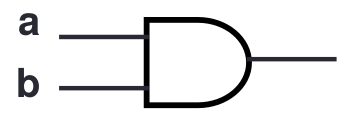
\includegraphics[width=.1\linewidth]{and} & $a \cdot b$ \\ \hline
		OR		& 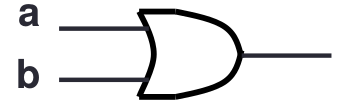
\includegraphics[width=.1\linewidth]{or}
	& $a+b$ \\ \hline
		NOT		&	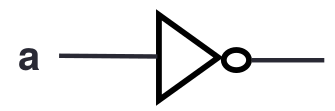
\includegraphics[width=.1\linewidth]{not}
	& $a'$ \\ \hline
	\end{tabular}	
	\begin{tabular}{|l|l|l|}
		\hline
		NAND	&	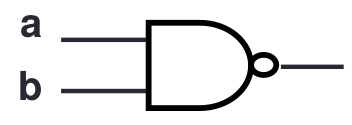
\includegraphics[width=.1\linewidth]{nand}
		&	$(a\cdot b)'$ \\ \hline
		NOR		&	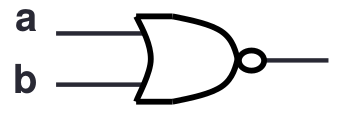
\includegraphics[width=.1\linewidth]{nor}
		& $(a+b)'$ \\ \hline
		XOR		&	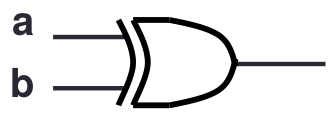
\includegraphics[width=.1\linewidth]{xor}
		& $a\oplus b$ \\ \hline
	\end{tabular}
	
	Note: $a\oplus b = (a\cdot b')+(a'\cdot b) = (a+b)\cdot(a\cdot b)'$
	
	\subsection{Universal Gates}
	\begin{itemize}
		\item \{NAND\} is a complete set of logic.\\
		\textbf{NOT}: $(x\cdot x)'=x'$, \textbf{AND}: $((x\cdot y	)'\cdot (x\cdot y)')'=((x\cdot y)')'=x\cdot y$,\\
		\textbf{OR}: $((x\cdot x)'\cdot(y.y)')'=(x'\cdot y')'=(x')'+(y')'=x+y$
		\item \{NOR\} is a complete set of logic.\\
		\textbf{NOT}: $(x+x)' = x'$, \textbf{AND}: $((x+x)'+(y+y)')' = (x'+y')'=(x')'\cdot (y')'=x\cdot y$, \textbf{OR}: $((x+y)'+(x+y)')'=((x+y)')' = x+y$
	\end{itemize}
	
	\section{Simplification}
	\subsection{Gray Code / Reflected Binary Code}
	\begin{itemize}
		\item Only a single bit differs from one code value to the next.
	\end{itemize}
	0000 -> 0001 -> 0011 -> 0010 -> 0110 -> 0111 -> 0101 -> 0100 -> 1100 -> 1101 -> 1111 -> 1110 -> 1010 -> 1011 -> 1001 -> 1000
	
	\subsection{K-maps}
	\begin{itemize}
		\item Labelled using gray code sequence.
		\item Recognise a group of size $2^n$, including wrapovers.
		\item \textbf{Prime Implicant}: the biggest grouping possible (product term)
		\item \textbf{Essential Primt Implicant}: a PI that includes at least one minterm not covered by any other PI.
		\item Don't care -- denoted with X
	\end{itemize}
	
	\section{Combinatorial Circuits (Stateless)}
	\subsection{Gate level design}
	\begin{descitemize}
		\item [Half-Adder] $C = X \cdot Y$, $S = X \oplus Y$
		\item [Full-adder] $C_{out} = X \cdot Y + (X \oplus Y) \cdot C_{in}$, $S=X\oplus(Y\oplus Z)=(X\oplus Y)\oplus Z$
		\item 4-bit parallel adder by cascading 4 full-adders via their carries
		\item [6-person voting system]: Using 2 full-adders, each input for each vote. Result tallied using a parallel adder.
		\item [Magnitude Comparator]: \textbf{input}: 2 unsigned values $A$ and $B$, \textbf{output}: "$A>B$", "$A=B$", "A<B"
	\end{descitemize}
	
	\subsection{Circuit Delays}
	\begin{itemize}
		\item For each component, time = max($\forall t_{input}) + t_\text{current component}$
		\item Propagation delay of ripple-carry parallel adders $\propto$ no. of bits
	\end{itemize}
	
	\section{MSI Components}
	\subsection{Decoders}
	E.g. 2x4 decoder, $F_0=X'\cdot Y'$, $F_1=X'\cdot Y$, $F_2=X\cdot Y'$, $F_3=X\cdot Y$
	
	\begin{tabular}{| l l | l l l l |}
		\hline
		$X$	& $Y$ & $F_0$ & $F_1$ & $F_2$ & $F_3$ \\ \hline
		0 & 0 & \textbf{1} & 0 & 0 & 0 \\
		0 & 1 & 0 & \textbf{1} & 0 & 0 \\
		1 & 0 & 0 & 0 & \textbf{1} & 0 \\
		1 & 1 & 0 & 0 & 0 & \textbf{1} \\
		\hline
	\end{tabular}
	\begin{tabular}{l}
	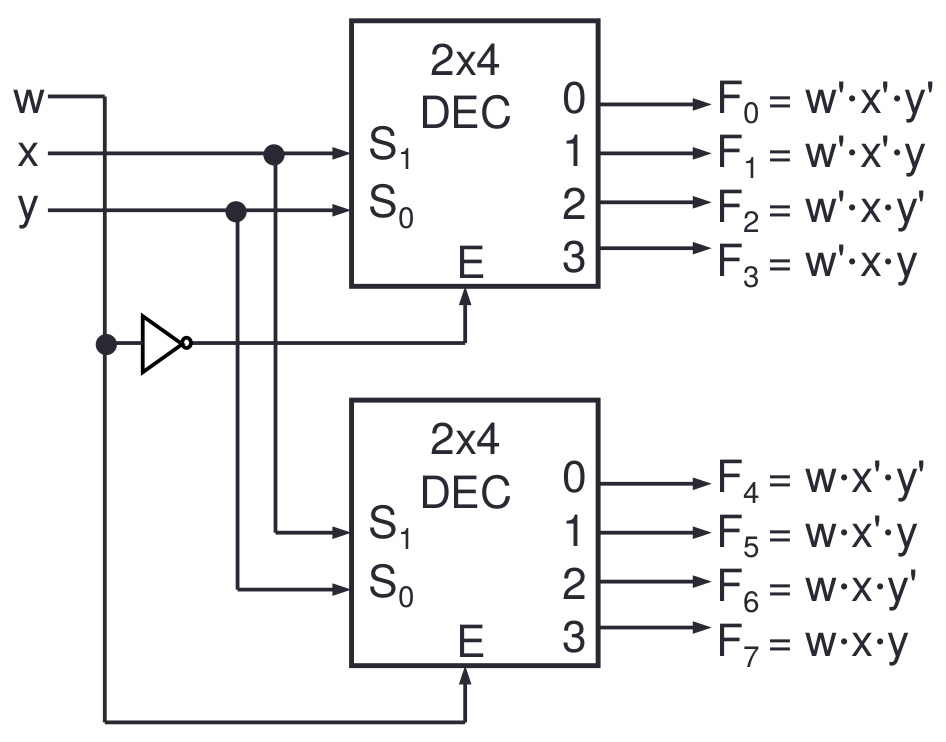
\includegraphics[width=0.35\linewidth]{larger-decoder}
	\end{tabular}
	\begin{itemize}
		\item Larger decoders can be constructed from smaller ones.
		\item In general, for an $n$-bit code, a decoder could select up to $2^n$ lines.
		\item Also exists decoders with enable. $E=0 \rightarrow F_0, F_1, F_2, F_3 = 0$
		\item Any combinatorial circuits with $n$ inputs, $m$ outputs can be implemented with an $n:2^n$ decoder with $m$ logic gates.
		\item Find sum-of-minterms, use each output of decoder corresponding to minterm/maxter as input to logic gate(s).
		\item Gate to use: Active-high: \textbf{OR} (minterm) \textbf{NOR} (maxterm), active-low: \textbf{NAND} (minterm) \textbf{AND} (maxterm)
	\end{itemize}
	
	\subsection{Encoders}
	\begin{itemize}
		\item 4-to-2 encoder, $D_0 = F_1 + F_3$, $D_1=F_2+F_3$
		\item 8-to-3 encoder, $x=D_4+D_5+D_6+D_7$, $y=D_2+D_3+D_6+D_7$, $z=D_1+D_3+D_5+D_7$
	\end{itemize}
	
	\textbf{8-to-3 encoder}
	\begin{tabular}{|l l l l | l l |}
		\hline
		$F_0$ & $F_1$ & $F_2$ & $F_3$ & $D_1$ & $D_0$ \\ \hline
		1 & 0 & 0 & 0 & 0 & 0 \\
		0 & 1 & 0 & 0 & 0 & 1 \\
		0 & 0 & 1 & 0 & 1 & 0 \\
		0 & 0 & 0 & 1 & 1 & 1 \\
		\hline
		\multicolumn{4}{|l|}{otherwise} & X & X \\ \hline
	\end{tabular}
	
	\textbf{Priority encoder}
	\begin{tabular}{| l l l l | l l l |}
		\hline
		$F_0$ & $F_1$ & $F_2$ & $F_3$ & $D_1$ & $D_0$ & $V$ \\ \hline
		0 & 0 & 0 & 0 & X & X & 0 \\
		1 & 0 & 0 & 0 & 0 & 0 & 1 \\
		X & 1 & 0 & 0 & 0 & 1 & 1 \\
		X & X & 1 & 0 & 1 & 0 & 1 \\
		X & X & X & 1 & 1 & 1 & 1 \\
		\hline
	\end{tabular}
	
	\subsection{Demultiplexers}
	\textbf{1-to-4 demultiplexer}
	
	\begin{tabular}{|l l|l l l l|}
		\hline
		$S_1$ & $S_0$ & $Y_0$ & $Y_1$ & $Y_2$ & $Y_3$ \\ \hline
		0 & 0 & D & 0 & 0 & 0 \\
		0 & 1 & 0 & D & 0 & 0 \\
		1 & 0 & 0 & 0 & D & 0 \\
		1 & 1 & 0 & 0 & 0 & D \\
		\hline
	\end{tabular}
	\begin{tabular}{l}
		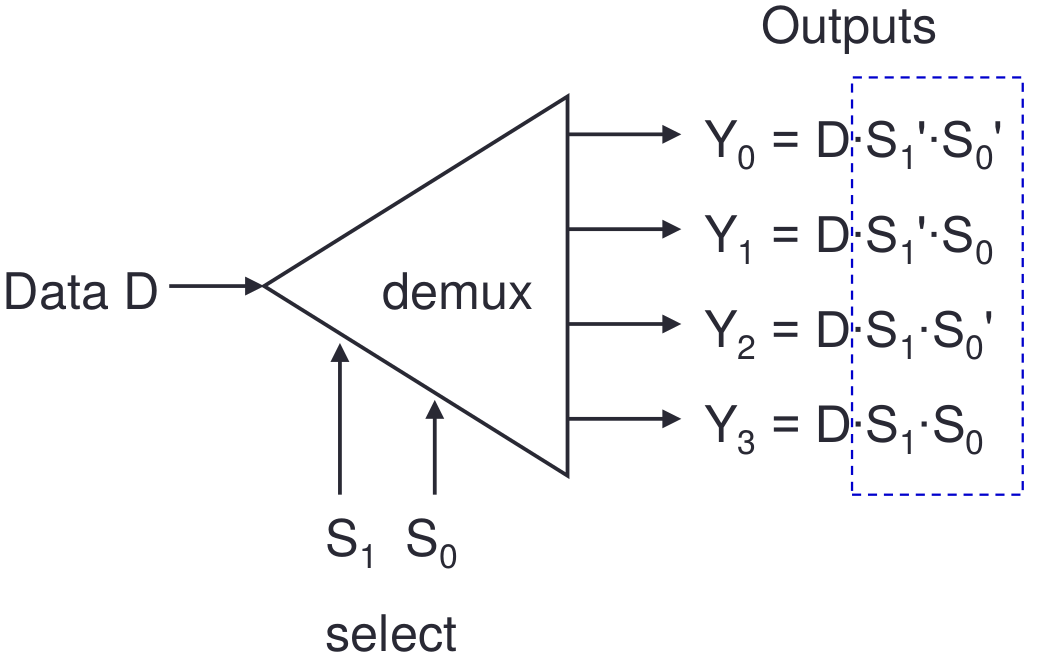
\includegraphics[width=0.4\linewidth]{demux}
	\end{tabular}
	\begin{itemize}
		\item Demux circuit is identical to a decoder w/ enable (data -> enable).
	\end{itemize}
	
	\subsection{Multiplexers}
	4-to-1 multiplexer
	
	\begin{tabular}{|l l|l|}
		\hline
		$S_1$ & $S_0$ & Y \\ \hline
		0 & 0 & $I_0$ \\
		0 & 1 & $I_1$ \\
		1 & 0 & $I_2$ \\
		1 & 1 & $I_3$ \\
		\hline
	\end{tabular}
	\begin{tabular}{l}
		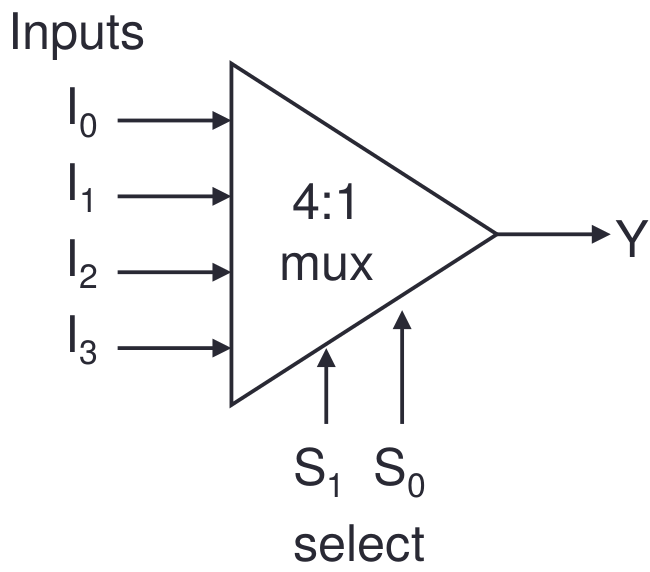
\includegraphics[width=0.25\linewidth]{mux}
		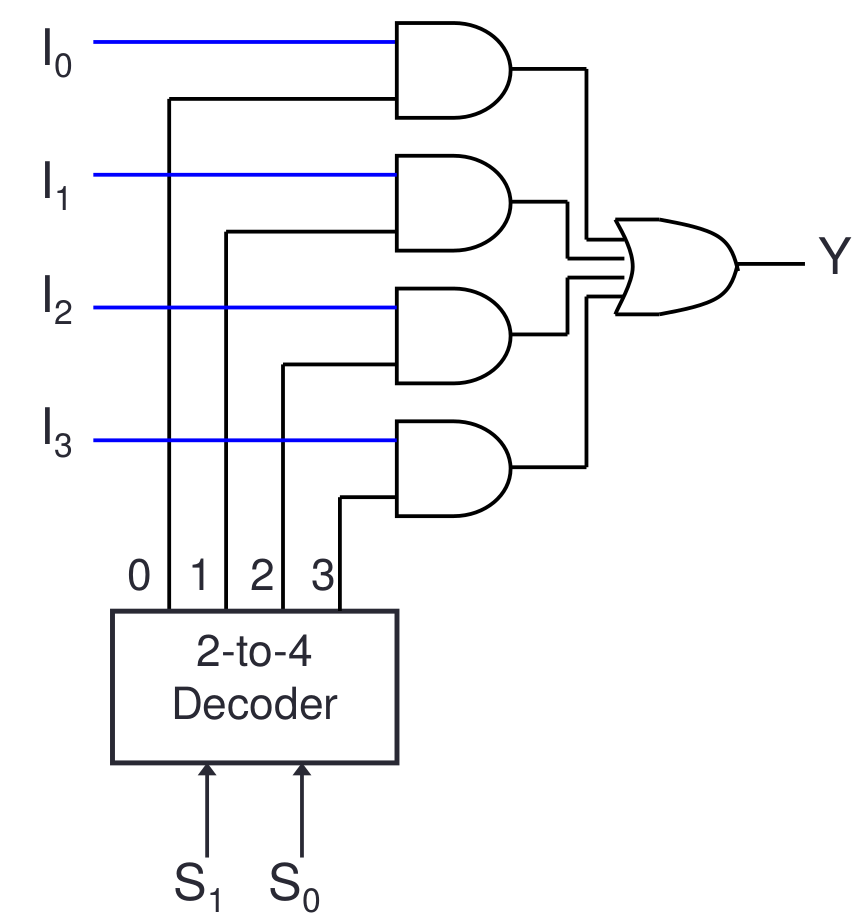
\includegraphics[width=0.2\linewidth]{mux1}
		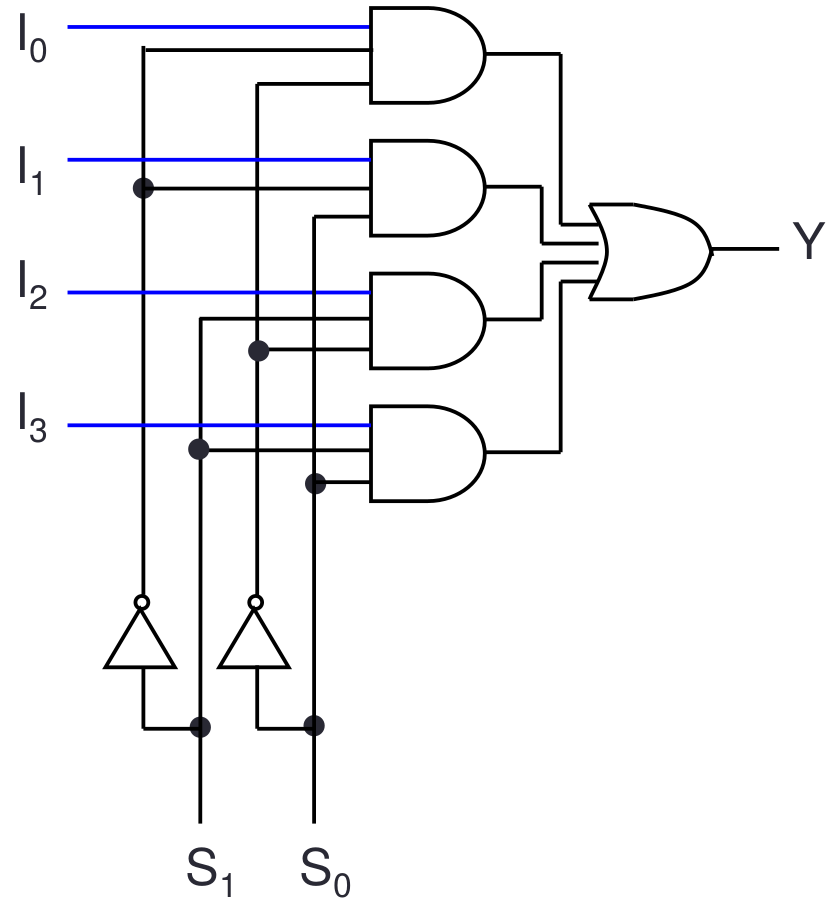
\includegraphics[width=0.2\linewidth]{mux2}
	\end{tabular}
	
	\begin{itemize}
		\item $Y=I_0\cdot(S_1'\cdot S_0') + I_1\cdot (S_1'\cdot S_0)+I_2\cdot(S_1\cdot S_0')+I_3\cdot(S_1\cdot S_0)$
		\item In minterms, $Y=I_0\cdot m_0 + I_1\cdot m_1 + I_2 \cdot m_2 + I_3 \cdot m_3$
		\item Possible to construct larger multiplexers from smaller ones.
	\end{itemize}
	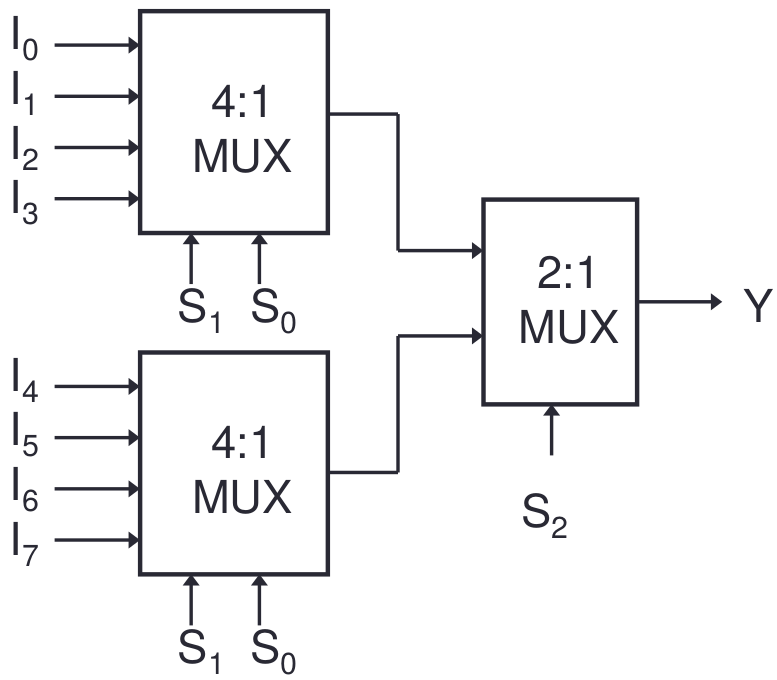
\includegraphics[width=0.3\linewidth]{mux3}
	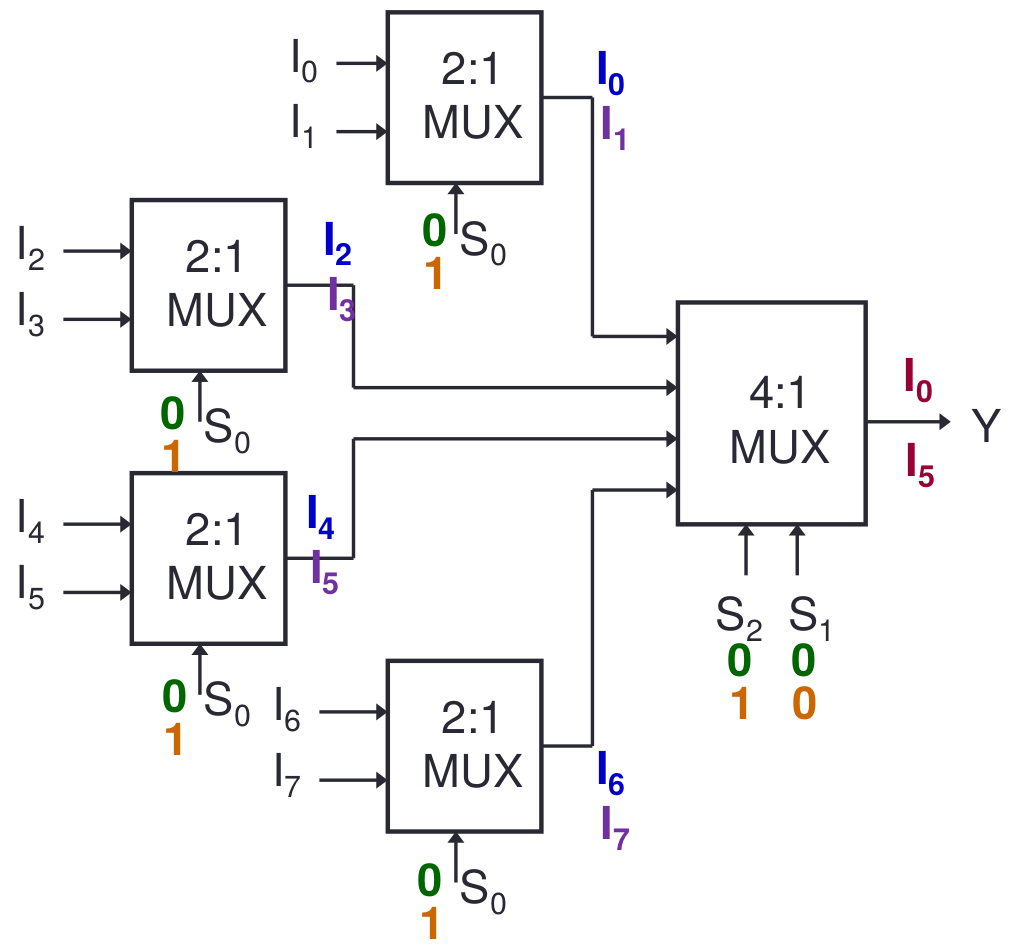
\includegraphics[width=0.35\linewidth]{mux4}
	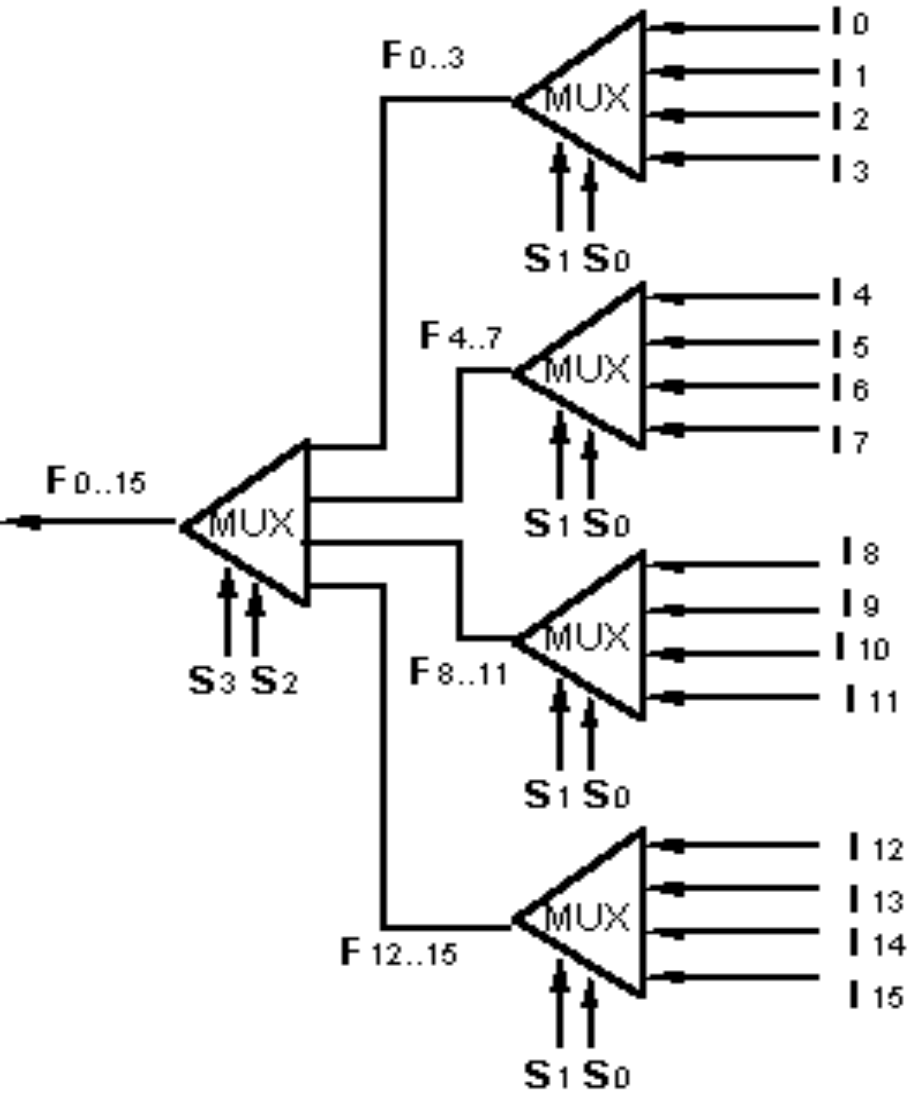
\includegraphics[width=0.3\linewidth]{mux5}
	\begin{itemize}
		\item Implement function using a $2^n$-to-1 multiplexer: put '1' on the data for each minterm, '0' otherwise. Connect input to selector.
		\item Can also use a \underline{single} smaller $2^{n-1}$-to-1 multiplexer: reserve one of the input vars in data line, the rest for selection. Group input by selection line values in truth table.
	\end{itemize}
	
	\section{Sequential Logic (Stateful)}
	\subsection{S-R Latch}
	\begin{tabular}{l}
		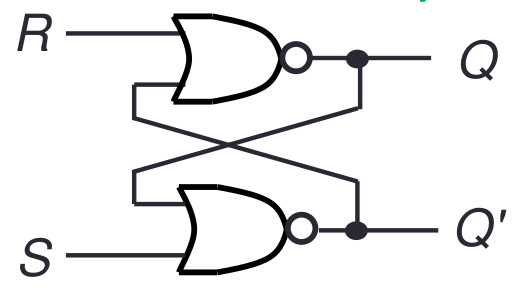
\includegraphics[width=0.25\linewidth]{s-r}
	\end{tabular}
	\begin{tabular}{|l l|l l|}
		\hline
		S & R & \multicolumn{2}{l|}{Q(t+1)} \\ \hline
		0 & 0 & Q(t) & No change \\
		0 & 1 & 0 & Reset \\
		1 & 0 & 1 & Set \\
		1 & 1 & \multicolumn{2}{l|}{indeterminate} \\
		\hline
	\end{tabular}
	
	\subsection{D Latch}
	\begin{tabular}{l}
		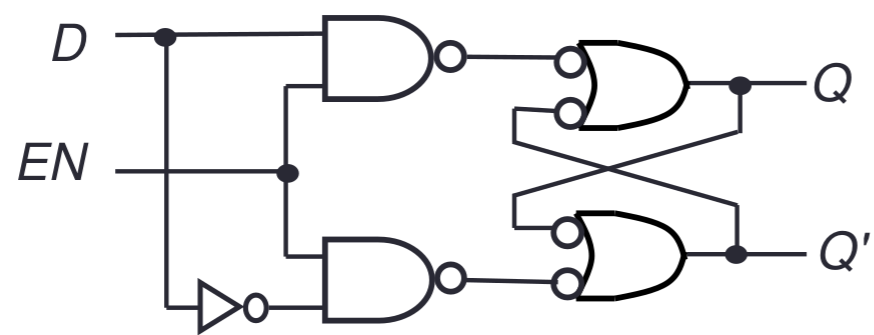
\includegraphics[width=0.3\linewidth]{d}
	\end{tabular}
	\begin{tabular}{|l l|l l|}
		\hline
		EN & D & \multicolumn{2}{l|}{Q(t+1)} \\ \hline
		1 & 0 & 0 & Reset \\
		1 & 1 & 1 & Set \\
		0 & X & Q(t) & No change \\
		\hline
	\end{tabular}
	
	\subsection{S-R Flip-flop}
	\begin{tabular}{l}
		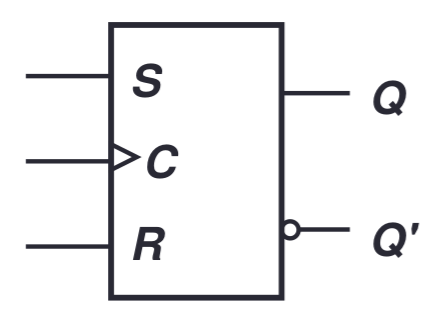
\includegraphics[width=0.2\linewidth]{sr}
	\end{tabular}
	\begin{tabular}{|l l l|l l|}
		\hline
		S & R & CLK & \multicolumn{2}{l|}{Q(t+1)} \\ \hline
		0 & 0 & X & Q(t) & No change \\
		0 & 1 & $\uparrow$ & 0 & Reset \\
		1 & 0 & $\uparrow$ & 1 & Set \\
		1 & 1 & $\uparrow$ & ? & Invalid \\
		\hline
	\end{tabular}
	
	\subsection{D Flip-Flop}
	\begin{tabular}{l}
		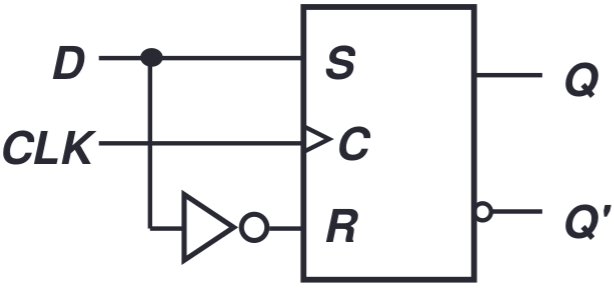
\includegraphics[width=0.2\linewidth]{d2}
	\end{tabular}
	\begin{tabular}{|l l|l l|}
		\hline
		D & CLK & \multicolumn{2}{l|}{Q(t+1)} \\ \hline
		1 & $\uparrow$ & 1 & Set \\
		0 & $\uparrow$ & 0 & Reset \\
		\hline
	\end{tabular}
	
	\subsection{J-K Flip-Flop }
	\begin{tabular}{l}
		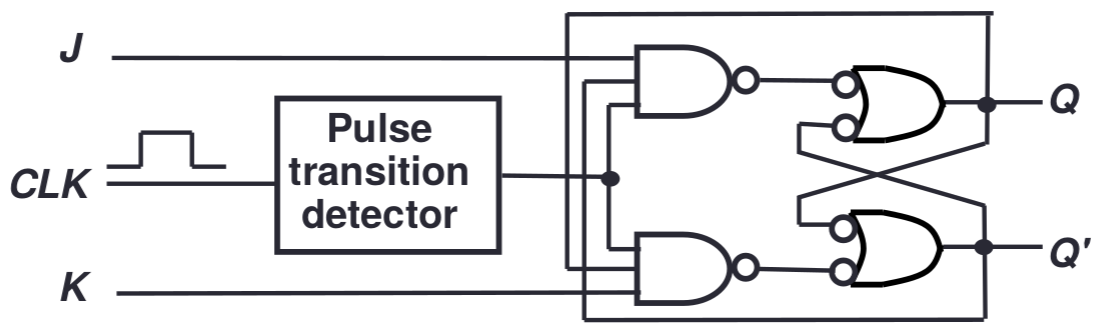
\includegraphics[width=0.42\linewidth]{jk}
	\end{tabular}
	\begin{tabular}{|l l|l l|}
		\hline
		J & K & \multicolumn{2}{l|}{Q(t+1)} \\ \hline
		0 & 0 & Q(t) & No change \\
		0 & 1 & 0 & Reset \\
		1 & 0 & 1 & Set \\
		1 & 1 & Q(t)' & Toggle \\
		\hline
	\end{tabular}
	
	\hspace*{\fill}All CLK $\uparrow$
	
	\subsection{T Flip-Flop}
	\begin{tabular}{l}
		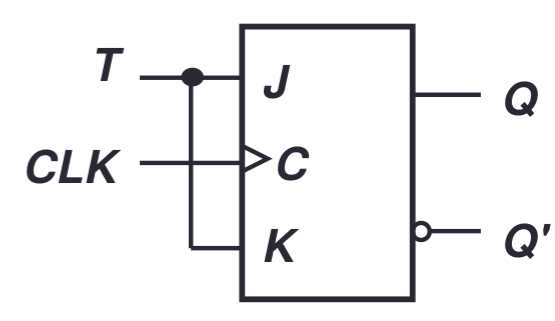
\includegraphics[width=0.2\linewidth]{t}
	\end{tabular}
	\begin{tabular}{|l l|l l|}
		\hline
		T & CLK & \multicolumn{2}{l|}{Q(t+1)} \\ \hline
		0 & $\uparrow$ & Q(t) & No change \\
		1 & $\uparrow$ & Q(t)' & Toggle \\
		\hline
	\end{tabular}
	
	\subsection{Flip-Flop Excitation Tables}
	\begin{tabular}{|l l|l l|}
		\multicolumn{4}{l}{\textbf{J-K Flip-Flop}} \\ \hline
		$Q$ & $Q^+$ & J & K \\ \hline
		0 & 0 & 0 & X \\
		0 & 1 & 1 & X \\
		1 & 0 & X & 1 \\
		1 & 1 & X & 0 \\
		\hline
	\end{tabular}\hfil
	\begin{tabular}{|l l|l l|}
		\multicolumn{4}{l}{\textbf{S-R Flip-Flop}} \\ \hline
		$Q$ & $Q^+$ & S & R \\ \hline
		0 & 0 & 0 & X \\
		0 & 1 & 1 & 0 \\
		1 & 0 & 0 & 1 \\
		1 & 1 & X & 0 \\
		\hline
	\end{tabular}
	
	\begin{tabular}{|l l|l|}
		\multicolumn{3}{l}{\textbf{D Flip-Flop}} \\ \hline
		$Q$ & $Q^+$ & D \\ \hline
		0 & 0 & 0 \\
		0 & 1 & 1 \\
		1 & 0 & 0 \\
		1 & 1 & 1 \\
		\hline
	\end{tabular}
	\begin{tabular}{|l l|l|}
		\multicolumn{3}{l}{\textbf{T Flip-Flop}} \\ \hline
		$Q$ & $Q^+$ & D \\ \hline
		0 & 0 & 0 \\
		0 & 1 & 1 \\
		1 & 0 & 1 \\
		1 & 1 & 0 \\
		\hline
	\end{tabular}\hfil
	\begin{tabular}{l}
		\textbf{Async Inputs} \\
		PRE = HIGH $\rightarrow$ Q=HIGH\\
		CLR = HIGH $\rightarrow$ Q=LOW
		
	\end{tabular}
	
	
	\subsection{State Table \& State Diagram}
	\begin{tabular}{l}
		A, B (\textbf{Present State})\\
		x (\textbf{Input}) \\
		$A^+$, $B^+$ (\textbf{Next State})\\
		y (\textbf{Output})
	\end{tabular}
	\begin{tabular}{l}
		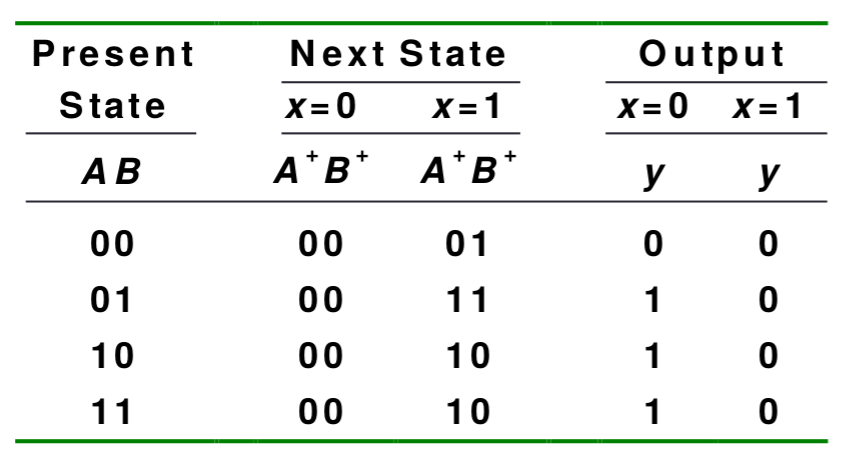
\includegraphics[width=0.3\linewidth]{state-diagram}
	\end{tabular}
	\begin{tabular}{l}
		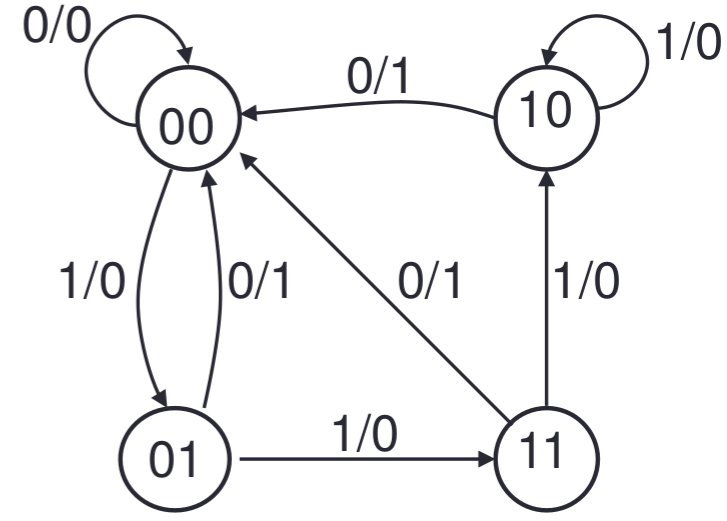
\includegraphics[width=0.22\linewidth]{state-diagram1}
	\end{tabular}
	
	
	\section{Pipelining}
	5 execution stages: (1) \textbf{IF} (Instruction Fetch), (2) \textbf{ID} (Instruction Decode \& Register Read), (3) \textbf{EX} (Execute / Calculate Address), (4) \textbf{MEM} (Access an operand in data memory), (5) \textbf{WB} (Write back result into a register)
	
	\subsection{Pipeline Datapath}
	Pipeline Registers store:
	\begin{itemize}
		\item \textbf{IF/ID} Instruction Read (including 2 Register Numbers for reading, 16-bit offset to be sign-extended to 32-bit); PC + 4
		\item \textbf{ID/EX} data values from register; 32-bit immediate value; PC + 4; Write Register Number
		\item \textbf{EX/ID} (PC + 4) + (Immediate $\times 4$); ALU result; \texttt{isZero?} signal; Data Read 2 from register; Write Register Number
		\item \textbf{MEM/WB} ALU result; Memory read data; Write Register Number
	\end{itemize}
	Grouping:
	\begin{itemize}
		\item \textbf{EX stage}: \texttt{RegDst, ALUSrc, ALUop}
		\item \textbf{MEM stage}: \texttt{MemRead, MemWrite, Branch}
		\item \textbf{WB stage}: \texttt{MemToReg, RegWrite}
	\end{itemize}
	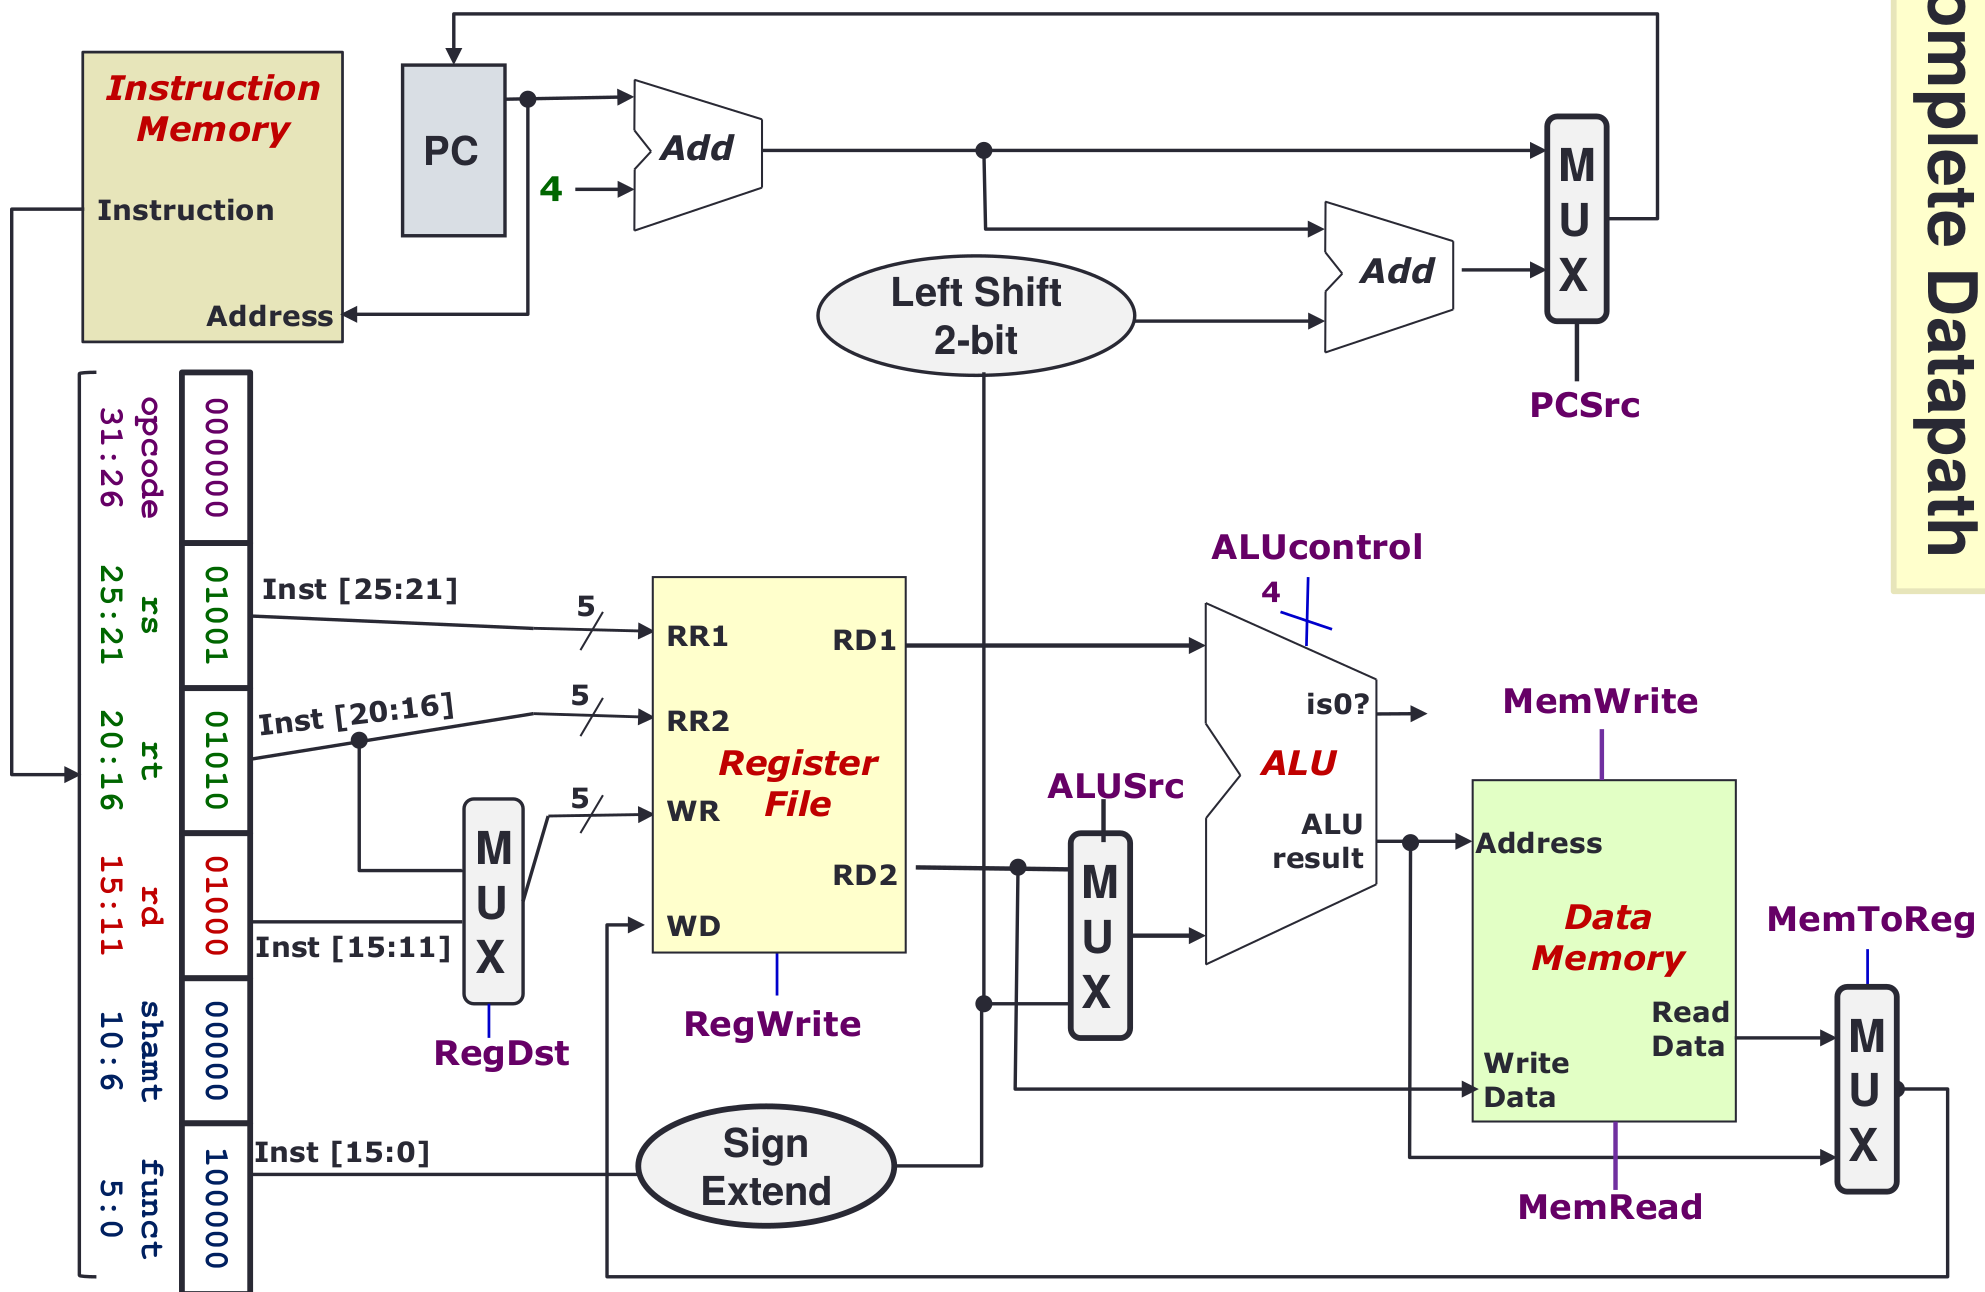
\includegraphics[width=0.9\linewidth]{datapath}
	
	\subsection{Performance calculations}	
	$T_k$ = Time for operation in stage $k$, $N$ = no of stages\\
	For $I$ instructions,	for total execution time ($time$) choose longest $CT$	
	\subsection{Single Cycle Processor Performance}
	Cycle Time: $CT_{seq}=\sum_{k=1}^{N}T_k$, $Time_{seq} = I \times CT_{seq}$
	\subsection{Multi-Cycle Processor Performance \textmd{(1 instruction many stages)}}
	$CT_{multi} = max(T_k)$, $Time_{multi} = I \times Average$ $CPI \times CT_{multi}$
	\subsection{Pipeline Processor}
	$CT_{pipeline} = max(T_k) + T_d$ ($T_d = $ overhead for pipelining)\\
	Cycles needed = $I + N - 1$ ($N-1$ cycles wasted filling up the pipeline)
	$Time_{pipeline} = (I + N - 1) \times (max(T_k) + T_d)$\\
	Speedup = $\frac{Time_{seq}}{Time_{pipeline}}$\\
	\textbf{Ideal case assumption}: every stage takes the same time ($\sum_{k=1}^{N}T_k=N\times T_k$), no pipeline overhead ($T_d=0$), $I$ much larger than $N$
	
	\subsection{Structural Hazard \textmd{(simultaneous use of a hardware resource)}}
	Soln: (1) \textbf{Stall} pipeline, (2) \textbf{Split} into \textbf{Data} \& \textbf{Instruction} memory
	\subsection{Data Dependency: RAW \textmd{(Read-after-Write)}}
	Solution: \textbf{Forwarding \& Bypass} (EX/MEM to ID/EX), but still problematic for LOAD instruction (need to stall)
	\subsection{Control Dependency}
	Decision only made in MEM stage (stall 3 cycles). Solution:
	\begin{enumerate}
		\item \textbf{Early Branch Resolution}, make decision in ID stage instead of MEM (but need dedicated adder), reduction 3 to 1 cycle delay, also add forward \& bypass ALU to ID stage for data dependency, still problematic for LOAD instruction.
		\item \textbf{Branch Prediction}, all branches assumed \textbf{not taken}. Correct guess no stall, wrong flush pipeline.
		\item \textbf{Delayed branch}, move $X$ non-control dependent instructions to after a branch as they are executed regardless of branch outcome. $X$ (branch-delay slot) = 1 for MIPS
	\end{enumerate}
	
	\section{Cache}
	\subsection{Memory Access Time}
	\textbf{Hit rate}, \textbf{Hit time} = cache access time, \textbf{miss rate} = 1 - hit rate, \textbf{miss penalty} = time to replace block cache + hit time\\
	\textbf{Average access time} = hit rate $\times$ hit time + miss rate $\times$ miss penalty.
	\subsection{Write Policy}
	\begin{itemize}
		\item \textbf{Write-through}, write data both to the cache \& main memory. Problem: write will operate at speed of main memory. Solution: write buffer b/w cache and main memory.
		\item \textbf{Write-back} cache, only write to cache, write to main memory only when cache block is replaced (evicted). Problem: wasteful to write back every evicted cache. Solution: Use a "dirty bit" if cache content is changed. Write back only if dirty bit is set.
	\end{itemize}
	\subsection{Types of Cache Misses}
	\textbf{Compulsory misses} on first access to a block, \textbf{Conflict misses} on collision, \textbf{Capacity misses} when blocks are discarded as cache is full
	\subsection{Handling Cache Misses}
	Read Miss: load data from memory to cache and then to register.
	Write miss:
	\begin{itemize}
		\item \textbf{Write-allocate}: load complete block to cache, change the required word in cache, write to main memory (write policy).
		\item \textbf{Write-around}: no loading to cache, write to main memory only
	\end{itemize}
	\subsection{Direct Mapped Cache \textmd{ -- (index, valid, tag)}}
	\textbf{How to id}: tag match with only 1 block.\\
	\textbf{Cache block size} = $2^N$ bytes, \textbf{no of cache blocks} = $2^M$\\
	\textbf{Offset} = $N$ bits, \textbf{Index} = $M$ bits, \textbf{Tag} = $32 - (N+M)$ bits
	\subsection{N-way Set Associative Cache}
	\textbf{How to id}: tag match for all the blocks within the set.\\
	A block maps to a unique set (each set having $n$ "cache blocks")\\
	\textbf{Cache block size} = $2^N$ bytes, \textbf{no of cache blocks} = $\frac{\text{size of cache}}{\text{size of block}}$,\\
	\textbf{no of sets} = $\frac{\text{no of blocks}}{\text{n in n-way}}$ = $2^M$,	\textbf{Offset} = $N$ bits, \textbf{Set Index} = $M$ bits
	\subsection{Fully Associative Cache \textmd{ -- capacity miss, \underline{no} conflict miss}}
	\textbf{How to id}: tag match for all the blocks in the cache.\\
	A memory block can be placed in any location in the cache.\\
	\textbf{Cache block size} = $2^N$ bytes, \textbf{no of cache blocks} = $2^M$\\
	\textbf{Offset} = $N$ bits, \textbf{Tag} = $32 - N$ bits (block number = tag)
	
	\subsection{Block Replacement Policy}
	\begin{itemize}
		\item \textbf{Least Recently Used (LRU)}: Replace the block which has not been accessed for the longest time. For temporal locality. \textbf{Problem:} hard to keep track if there are many choices.
		\item \textbf{FIFO}, \textbf{Random Replacement}, \textbf{Least Frequently Used}
	\end{itemize}
	
	\section{Performance}
	\subsection{Execution Time}
	Avg Cycle/Instruction: \textbf{CPI} = $\frac{(\text{CPU time} \times \text{clock rate})}{\text{Instruction count}} = \frac{\text{clock cycles}}{\text{instruction count}}$\\
	CPU time = ${seconds} = {instructions}\times\frac{cycles}{instruction}\times\frac{seconds}{cycle}$\\
	$CPI = \sum\limits_{k=1}^{n}(CPI_k\times F_k)$ where $F_k = \frac{I_k \text{(Instruction frequency)}}{\text{Instruction count}}$
	
	\subsection{Amdahl's Law}
	Performance uis limited to the non-speedup portion of the program.\\
	\textbf{Execution time after improvement} = Execution time of unaffected part + $\frac{\text{Execution time of affected part}}{\text{speedup}}$\\
	Corollary: Optimise the common case first!
	
	
	\section{Additional stuffs}
	Opcode -- maximise:	allocate 1 each to the shortest opcode types.\\
	Number of unusable bits: Type B=(32 - 29)=3, Type C=(32 - 16)=16\\
	No of type A = $2^{32} - 2^3 - 2^{16} + 2$ 
			
%		\begin{minted}{javascript}
		
%		\end{minted}
\end{multicols*}
\end{document}